\chapter{Andreev Bound State Current in SNS-junction}
We can use equation \eqref{JosephsonCurrent} and \eqref{FreeEnergy} to express the Josephson current in terms of the ABS energy and the phase difference.
\begin{equation}
\begin{split}
    I_x(\Delta \varphi) &= \sum_{k_y} \delta I(\fet{r},\fet{k}) \rightarrow \int dy \int \frac{dk_y}{2\pi} \delta I(\fet{r},\fet{k}),\\
    I_y(\Delta \varphi) &= \sum_{k_x} \delta I(\fet{r},\fet{k}) \rightarrow \int dx \int \frac{dk_x}{2\pi} \delta I(\fet{r},\fet{k}),\\
\end{split}
\label{TotalCurrent}
\end{equation}
where we have defined 
\begin{equation}
    \delta I(\fet{r},\fet{k}) \equiv -\frac{2e}{\hbar}\tanh\left(\frac{E_{\kbf}}{2k_BT}\right)\frac{\partial E_{\kbf}}{\partial (\Delta \varphi)}
    \label{Current5}
\end{equation}
and $I_y$ should be zero due to current conservation. The current density will be given as
\begin{equation}
\begin{split}
    j_x(x,y) &= \int \frac{dk_y}{2\pi} \delta I(\fet{r},\fet{k}) = \frac{k_F}{2\pi}\int d\theta_k \cos\theta_k \delta I(\fet{r},\fet{k}) ,\\
    j_y(x,y) &= \int \frac{dk_x}{2\pi} \delta I(\fet{r},\fet{k}) = \frac{k_F}{2\pi}\int d\theta_k \sin\theta_k \delta I(\fet{r},\fet{k}).\\
\end{split}
\label{CurrentDensity}
\end{equation}

\section{ABS current without barriers or applied field}
In the case with no barriers or magnetic field we use equation \eqref{AndreevEnergy1} in equation \eqref{Current5} to obtain
\begin{equation}
    \delta I = \frac{e\Delta_0}{\hbar}\sin\left(\frac{\Delta\varphi}{2}\right)\tanh\left(\frac{\Delta_0\cos(\Delta\varphi/2)}{2k_BT}\right),
\end{equation}
which we notice is independent of position and $\theta_k$. We find the current density to be zero in the $y$-direction, i.e. $j_y(x,y) = 0$. The current density along the $x$-axis is uniform $j_x(x,y) = I_x/W$, and the total current is
\begin{equation}
\begin{split}
   I_x = k_F W\frac{e\Delta_0}{\pi \hbar} \sin\left(\frac{\Delta\varphi}{2}\right)\tanh\left(\frac{\Delta_0\cos(\Delta\varphi/2)}{2k_BT}\right).
\end{split}
\label{TotalCurrent}
\end{equation}
In the high temperature regime $(k_BT \gtrsim \Delta_0)$ this can be approximated to
\begin{equation}
    I_x = k_F W\frac{e\Delta_0}{\pi \hbar} \sin\left(\frac{\Delta\varphi}{2}\right)\frac{\Delta_0\cos(\Delta\varphi/2)}{2k_BT} =\frac{ k_F W e\Delta_0^2}{4\pi \hbar k_BT}\sin \Delta \varphi
\end{equation}
and the high temperature critical current is
\begin{equation}
    I_{c,0} = \frac{k_F W e\Delta_0^2}{4\pi \hbar k_BT}.
\label{Ic0-highT}
\end{equation}


\section{ABS current with barriers}
In the case with barriers we obtained the ABS energy in equation in \eqref{AndreevEnergy2}, which give
\begin{equation}
\delta I = \frac{e \Delta_0}{2 \hbar}\frac{\sin(\Delta \varphi)}{\sqrt{(\cos^2(\Delta \varphi /2 )+ \zeta)(\zeta + 1)}}\tanh\left(\frac{\Delta_0}{2k_BT}\sqrt{\frac{\cos^2(\Delta \varphi/2) + \zeta}{\zeta + 1}}\right).
\end{equation}
Again the $\delta I $ is independent of position and $\theta$ such that the total current is simply
\begin{equation}
I_x = k_FW \frac{e \Delta_0}{2 \pi \hbar}\frac{\sin(\Delta \varphi)}{\sqrt{(\cos^2(\Delta \varphi /2 )+ \zeta)(\zeta + 1)}}\tanh\left(\frac{\Delta_0}{2k_BT}\sqrt{\frac{\cos^2(\Delta \varphi/2) + \zeta}{\zeta + 1}}\right).
\end{equation}
We find the high temperature critical current:
\begin{equation}
I_{c,\zeta} = \frac{k_F W e\Delta_0^2}{4\pi \hbar k_BT}\frac{1}{\zeta + 1} = \frac{I_{c,0}}{\zeta+1}.
\end{equation}

\begin{figure}[hhh]
\centering
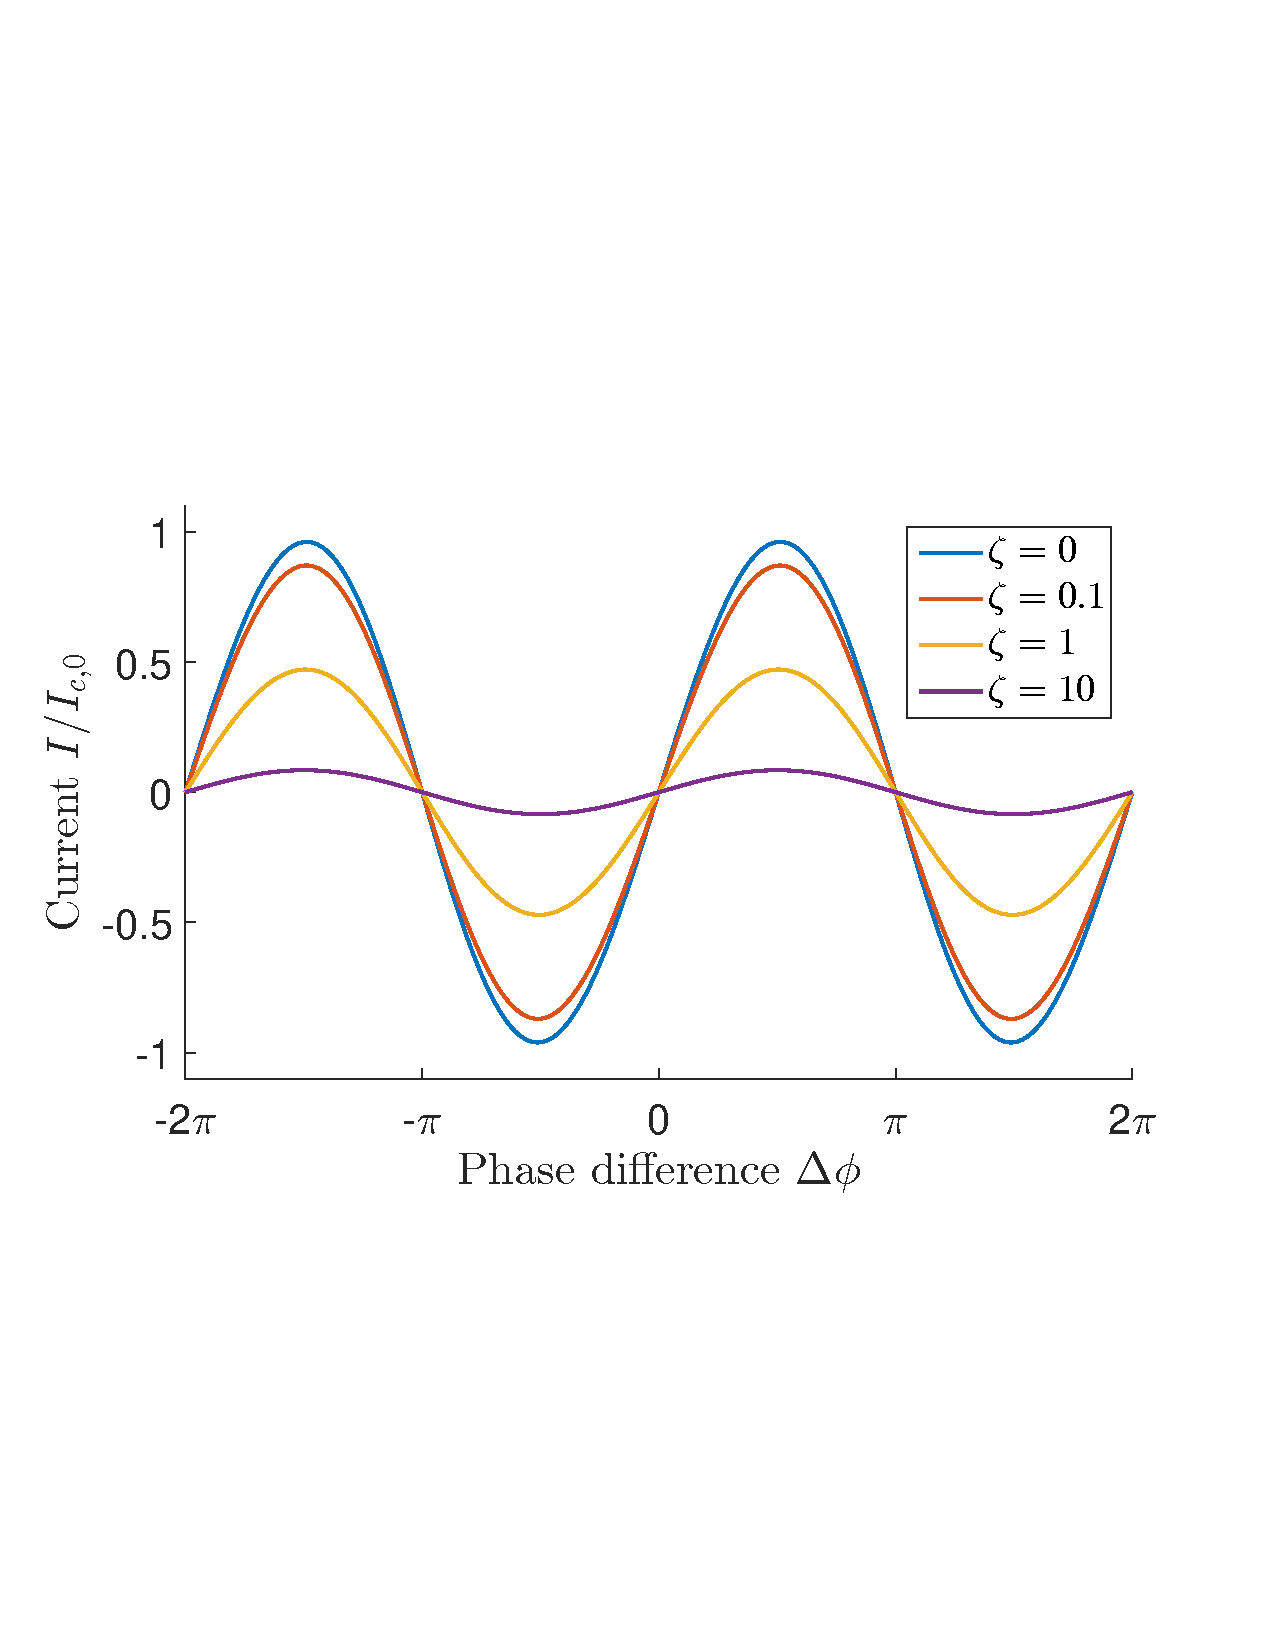
\includegraphics[width=12cm,clip=true,trim=0cm 7cm 1cm 7cm]{fig/WithoutField}
%\subfigure[]{\includegraphics[width=3.9cm]{Dustin}\label{fig:Dustin}}
%\hfill
%\subfigure[]{\includegraphics[width=3.45cm]{Martin}\label{fig:Martin}}
\caption{blabla}
\label{fig:motionEarth}
\end{figure}

\section{ABS current with constant applied field}
With no barriers, but magnetic field we find the current from the ABS energy in equation \eqref{AndreevEnergy3}:
\begin{equation}
    \delta I_k(\Delta \varphi) = \frac{e\Delta_0}{\hbar} \sin\left(\frac{\Delta \varphi}{2} - \frac{\gamma_k}{2}\right)\tanh\left(\frac{\Delta_0\cos\left(\frac{\Delta \varphi}{2} - \frac{\gamma_k}{2}\right)}{2k_BT}\right).
    \label{dIwithB}
\end{equation}
$\gamma_k$ will be dependent on the magnetic field, and on the trajectory of the particle. We will consider three different modulations of the magnetic field. That is constant magnetic field, and sinusoidal field along and transverse to the junction. We assume complete expulsion of the field in the superconducting region, due to the Meissner effect.

\subsection{Constant field}
\label{sec:ConstField}
We will first consider a constant magnetic field of strength $B$:
\begin{equation}
    \fet{B} = B\left[\Theta(x+L/2) - \Theta(x-L/2) \right]\hat{z}.
\end{equation}
We choose the gauge of the $\fet{A}$-field as
\begin{equation}
    \fet{A} = -By\left[\Theta(x+L/2) - \Theta(x-L/2) \right]\hat{x}.
\end{equation}
The Aharonov-Bohm phase shift, $\gamma(x_0,y_0,\theta_k)$, is calculated from equation \eqref{gamma} by integration along a path through the point $(x_0,y_0)$ at an angle $\theta_k$ with the $x$-axis, as shown in figure \ref{fig:Explaination}. The trajectory will be given by the line
\begin{equation}
    y(x) = y_0-x_0\tan\theta_k + x\tan\theta_k.
    \label{trajectory}
\end{equation}
Using this in equation \eqref{gamma} we find $\gamma$:
\begin{equation}
    \gamma = -\frac{2e}{\hbar}\int_L^R \fet{A}\cdot d\fet{l} = B\frac{2e}{\hbar}\int_{-L/2}^{L/2}y(x)dx = \frac{2L}{l_m^2}\left(y_0 - x_0\tan\theta_k \right)
\label{gamma1}
\end{equation}
with $l_m = \sqrt{\hbar/eB}$ as the magnetic length.
%If we assume $W$ to be much larger than $L$ we can ignore the boundaries along the junction, and the current will be conserved such that there will be no $x_0$ dependence. 
We use this expression in equation \eqref{dIwithB} and \eqref{CurrentDensity} to find the current density. The result is shown in figure \ref{fig:Constant} for three different magnetic lengths. 
\begin{figure}[hhh]
\centering
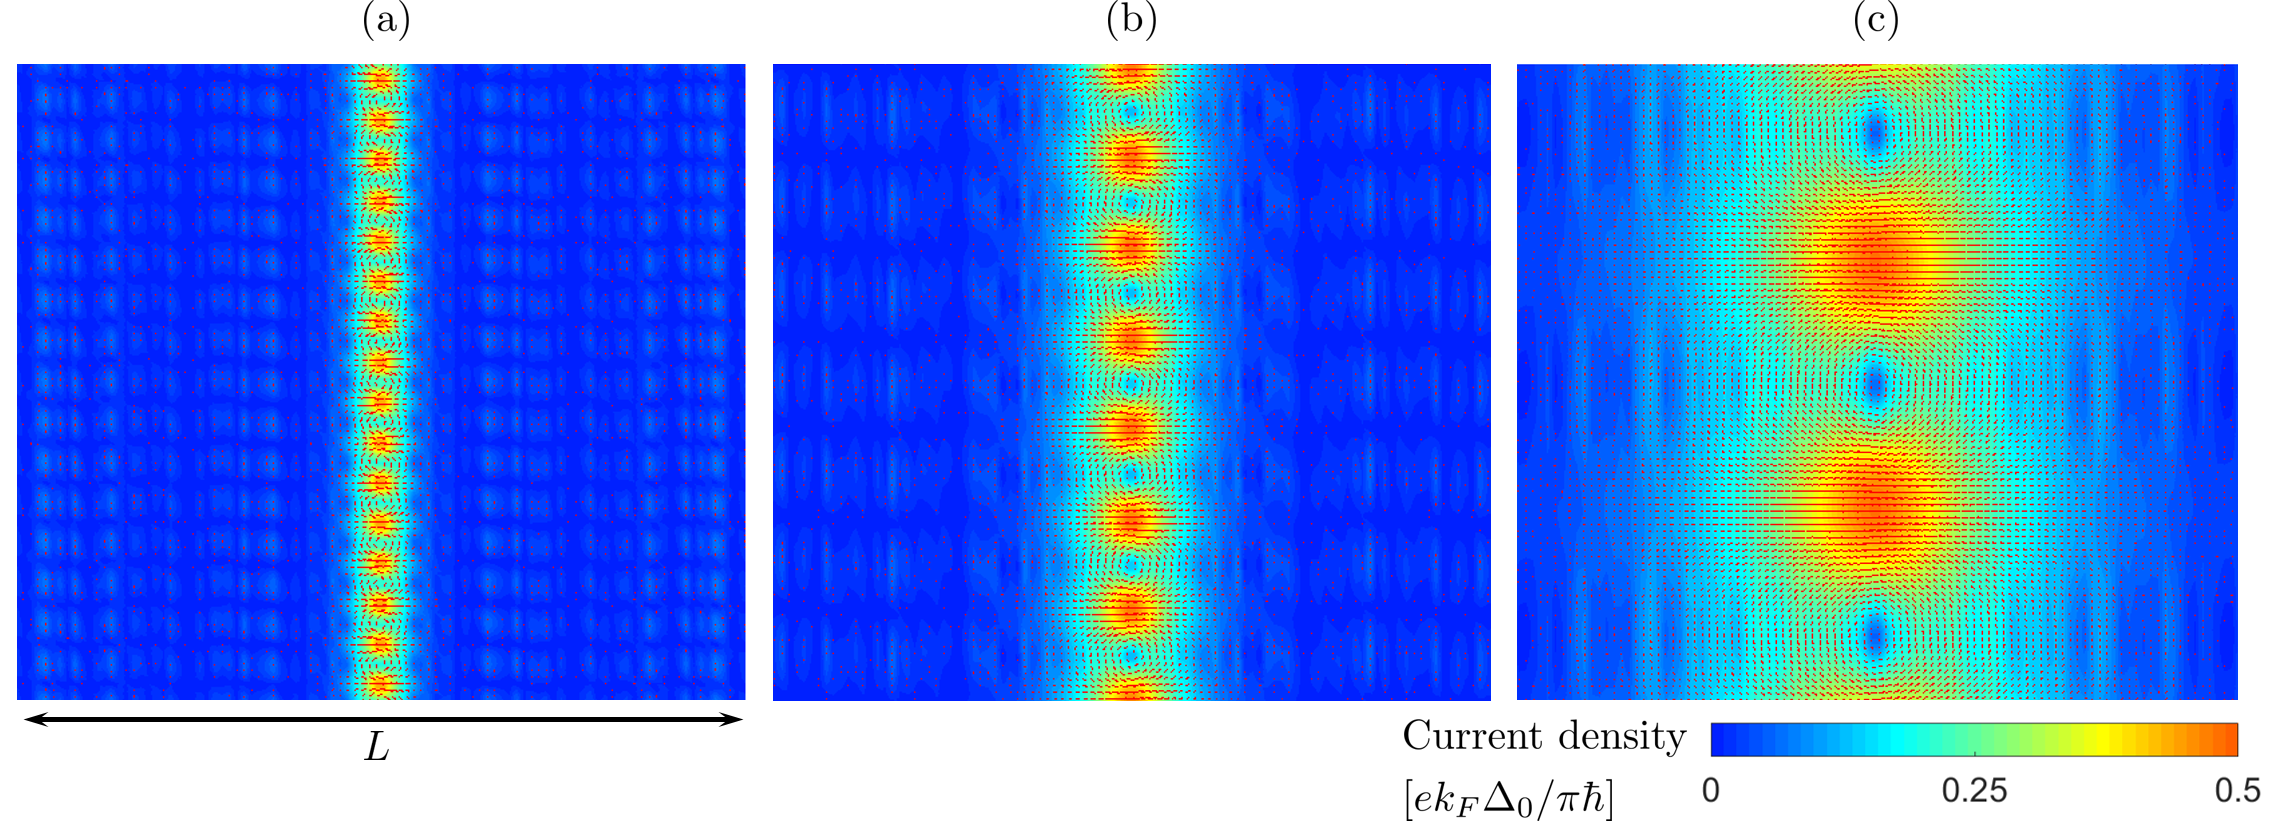
\includegraphics[width=17cm]{fig/dist1}
%\subfigure[]{\includegraphics[width=3.9cm]{Dustin}\label{fig:Dustin}}
%\hfill
%\subfigure[]{\includegraphics[width=3.45cm]{Martin}\label{fig:Martin}}
\caption{blabla}
\label{fig:Constant}
\end{figure}
\\
In order to find the total current we combine equation \eqref{TotalCurrent}, \eqref{CurrentDensity} and \eqref{dIwithB}:
\begin{equation}
I_x = \frac{k_F}{2\pi}\frac{e\Delta_0}{\hbar}\int_{-W/2}^{W/2}dy_0\int_{-\pi/2}^{\pi/2}d\theta_k\cos \theta_k \sin\left(\frac{\Delta \varphi}{2}-\frac{\gamma}{2}\right)\tanh\left(\frac{\Delta_0}{2k_BT}\cos\left(\frac{\Delta \varphi}{2}-\frac{\gamma}{2}\right)\right)
\end{equation}
which in the high temperature regime $(k_BT \gtrsim \Delta_0)$ can be simplified to
\begin{equation}
I_x = \frac{I_{c,0}}{2W}\int_{-W/2}^{W/2}dy_0\int_{\pi/2}^{\pi/2} d\theta_k \cos \theta_k \sin (\Delta \varphi - \gamma ).
\label{TotalCurrentHighT}
\end{equation}
From equation \eqref{gamma1} we notice that $\gamma(x_0,y_0,\theta_k) = -\gamma(x_0,-y_0,-\theta)$ which allows us to write
\begin{equation}
I_x = \frac{I_{c,0}}{W}\sin(\Delta \varphi) \int_{-W/2}^{W/2}dy_0\int_0^{\pi/2} d\theta_k\cos \theta_k \cos\gamma.
\end{equation}
The integral over $y_0$ gives in the low field regime $(l_m \gg L)$
\begin{equation}
\int_{-W/2}^{W/2}dy_0\cos\gamma = \frac{l_m^2}{L}\sin\left(\frac{LW}{l_m^2}\right)\cos\left(\frac{2L}{l_m^2}x_0\tan\theta_k\right) \approx \frac{l_m^2}{L}\sin\left(\frac{LW}{l_m^2}\right),
\end{equation}
and the total current is
\begin{equation}
I_x = I_{c,0}\frac{\sin\left(\frac{e}{\hbar}\Phi\right)}{\frac{e}{\hbar}\Phi}\sin \Delta \varphi
\end{equation}
with $\Phi = BLW$ as the magnetic flux. The critical current is the well known Fraunhofer oscillations
\begin{equation}
I_{c,\mathrm{const}} = I_{c,0} \frac{\sin\left(\frac{e}{\hbar}\Phi\right)}{\frac{e}{\hbar}\Phi}.
\end{equation}
This result is shown in figure \ref{fig:Fraunhofer}.
\begin{figure}[hhh]
\centering
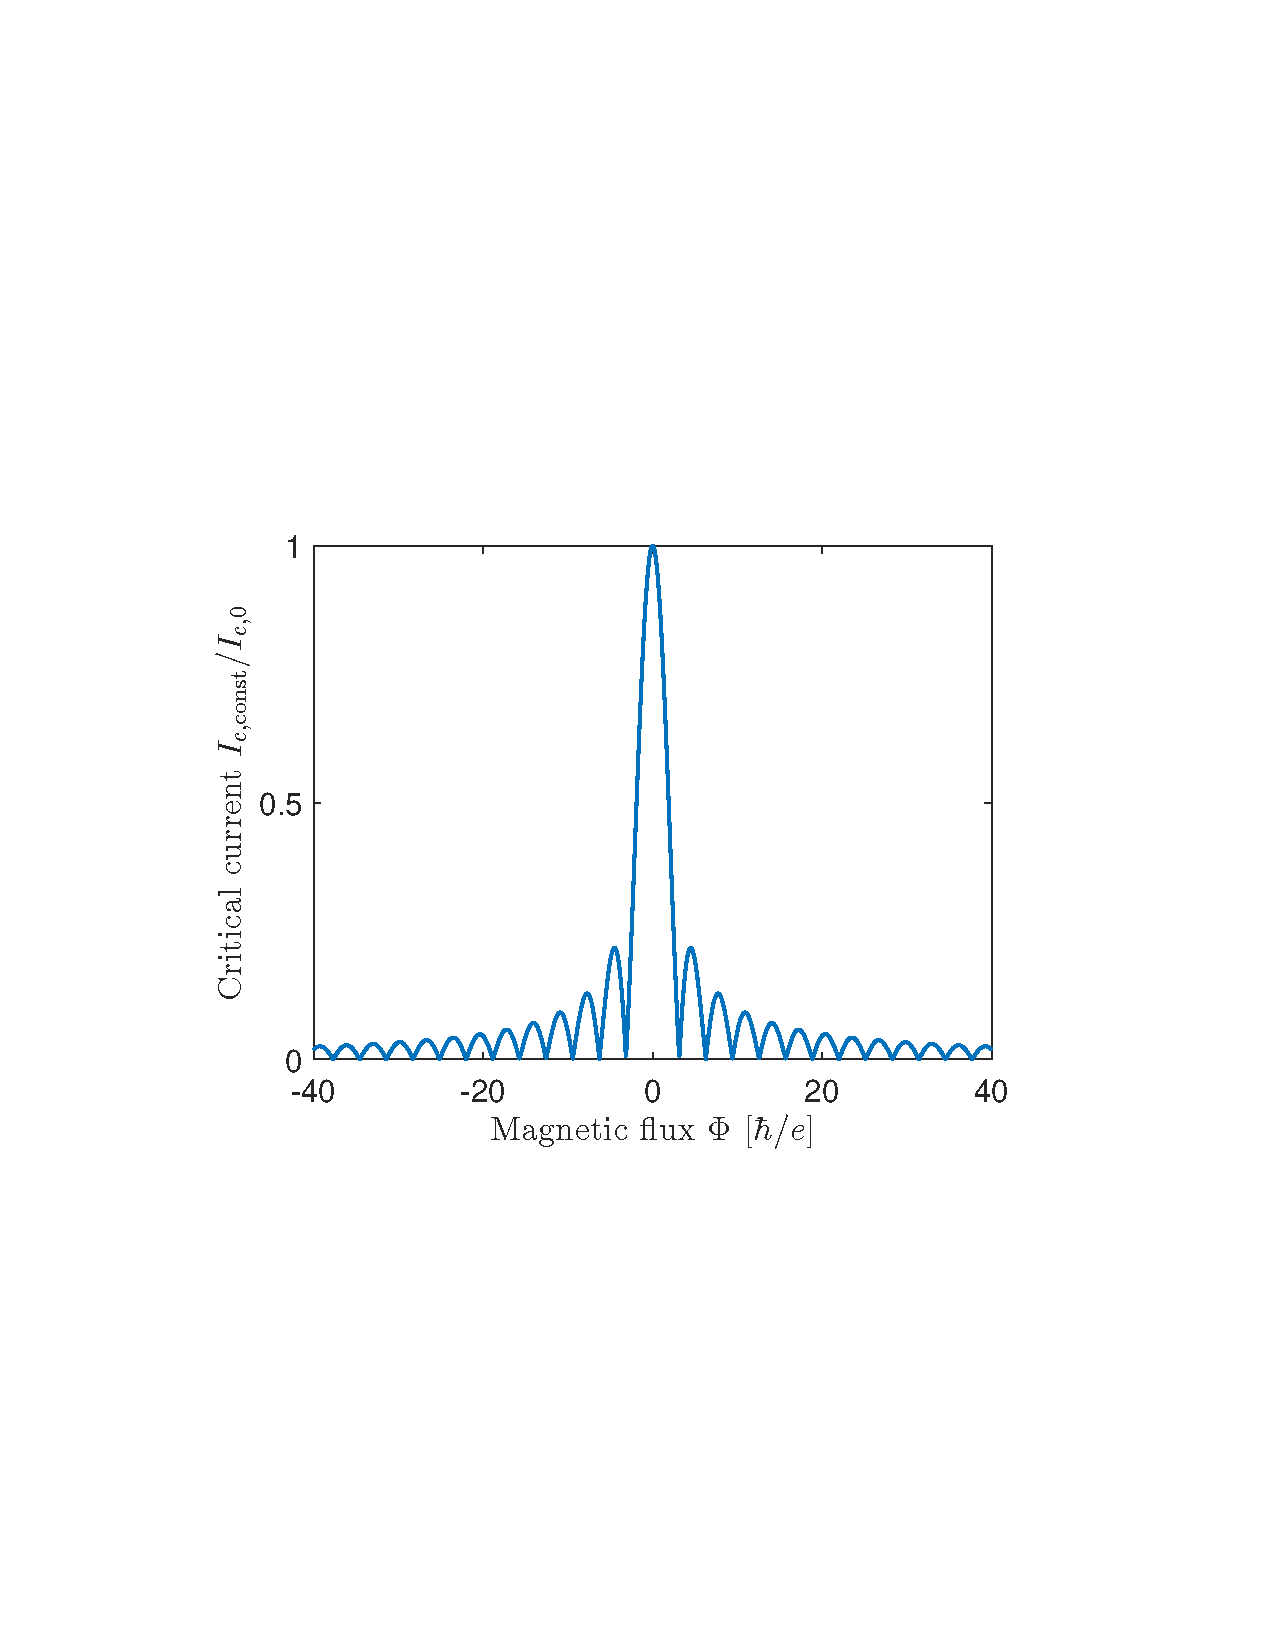
\includegraphics[width=12cm,clip=true,trim=3cm 8cm 3cm 8cm]{fig/Fraunhofer}
%\subfigure[]{\includegraphics[width=3.9cm]{Dustin}\label{fig:Dustin}}
%\hfill
%\subfigure[]{\includegraphics[width=3.45cm]{Martin}\label{fig:Martin}}
\caption{blabla}
\label{fig:Fraunhofer}
\end{figure}
\\
\subsection{Sinusoidal field varying along the junction}
We will next consider a sinusoidal magnetic field along the junction:
\begin{equation}
    \fet{B} = B\sin\left(\frac{2\pi}{\lambda}x + \varphi\right)\left[\Theta(x+L/2) - \Theta(x-L/2) \right]\hat{z}
\end{equation}
with the gauge
\begin{equation}
    \fet{A} = -By\sin\left(\frac{2\pi}{\lambda}x + \varphi\right)\left[\Theta(x+L/2) - \Theta(x-L/2) \right]\hat{x}.
\end{equation}
Again we find $\gamma(x_0,y_0,\theta_k)$ using equation \eqref{gamma} and integrating along the trajectory in \eqref{trajectory}:
\begin{equation}
\begin{split}
    \gamma &= \frac{2}{l_m^2}\int_{-L/2}^{L/2}y(x)\sin\left(\frac{2\pi}{\lambda} +\varphi \right) dx \\
    &= \frac{2\lambda}{\pi l_m^2}\left(\left[y_0 - x_0\tan\theta_k\right]\sin\left(\frac{\pi L}{\lambda}\right)\sin\varphi+\frac{L}{2}\tan\theta_k\left[\frac{\lambda}{\pi L}\sin\left(\frac{\pi L}{\lambda}\right)-\cos\left(\frac{\pi L}{\lambda}\right)\right]\cos\varphi\right).
\end{split}
\label{gamma2}
\end{equation}

\subsubsection{Anti-symmetric field}
More specifically we may take $\varphi$ to zero, yielding
\begin{equation}
\gamma = \frac{L^2}{l_m^2}\tan\theta_k\left[\left(\frac{\lambda}{\pi L}\right)^2\sin\left(\frac{\pi L}{\lambda}\right)-\frac{\lambda}{\pi L}\cos\left(\frac{\pi L}{\lambda}\right)\right].
\end{equation}
We notice how $\gamma$ now is position-independent and expect a uniform current distribution. Using this expression in equation \eqref{dIwithB} and \eqref{CurrentDensity} the current density is found. The result is shown in figure \ref{fig:Dist3a} for varying wavelengths, $\lambda$, of the external field.
\\
\\
We find the total current in the high temperature regime as we did in the previous section. As $\gamma$ \eqref{gamma2} is indepenent of $y_0$, equation \eqref{TotalCurrentHighT} yields
\begin{equation}
I = \frac{I_{c,0}}{2}\int_{-\pi/2}^{\pi/2}d\theta_k\cos\theta_k\sin(\Delta \varphi - \gamma).
\end{equation}
Using that $\gamma(\theta_k) = -\gamma(-\theta_k)$ this can be rewritten to
\begin{equation}
I = I_{c,0}\sin\Delta\varphi\int_0^{\pi/2}d\theta_k\cos\theta_k\cos\gamma.
\end{equation}
After inserting for $\gamma$ and integrating over $\theta_k$ we obtain the total current:
\begin{equation}
I = I_{c,0}\sin\Delta\varphi\frac{L^2}{l_m^2}\left|f(\lambda)\right|K_1\left(\frac{L^2}{l_m^2}\left|f(\lambda)\right|\right)
\end{equation}
where $K_1(z)$ is the modified Bessel function of second kind and we have defined
\begin{equation}
f(\lambda) \equiv \left(\frac{\lambda}{\pi L}\right)^2\sin\left(\frac{\pi L}{\lambda}\right)-\frac{\lambda}{\pi L}\cos\left(\frac{\pi L}{\lambda}\right).
\end{equation}
Hence, the critical current is
\begin{equation}
    I_c = I_{c,0}\frac{L^2}{l_m^2}\left|f(\lambda)\right|K_1\left(\frac{L^2}{l_m^2}\left|f(\lambda)\right|\right).
\end{equation}
This result is shown in figure \ref{fig:Dist3c} for different wavelengths, $\lambda$, and varying magnetic field strength,$B$.
\begin{figure}[hhh]
\centering
%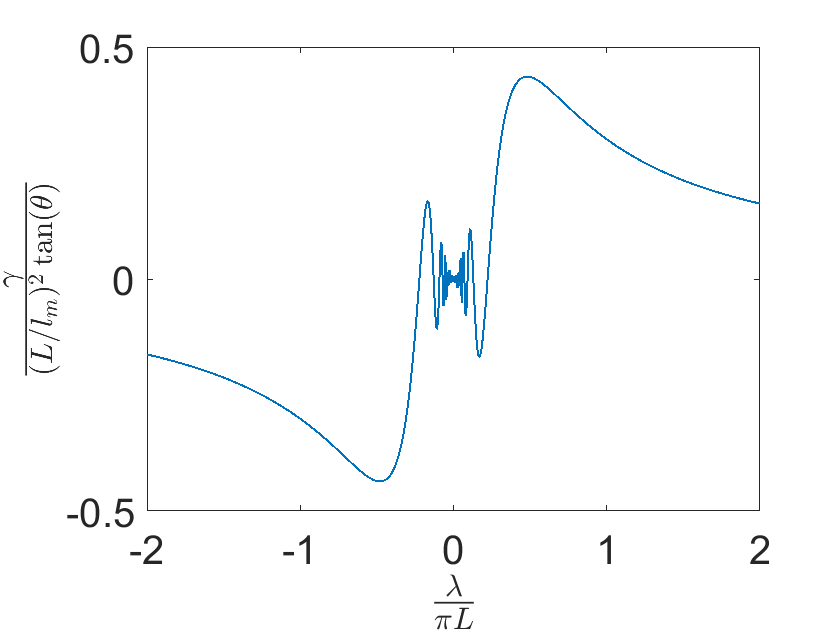
\includegraphics[width=10cm]{fig/1_Max3_l_0-3_phi_0}
\subfigure[]{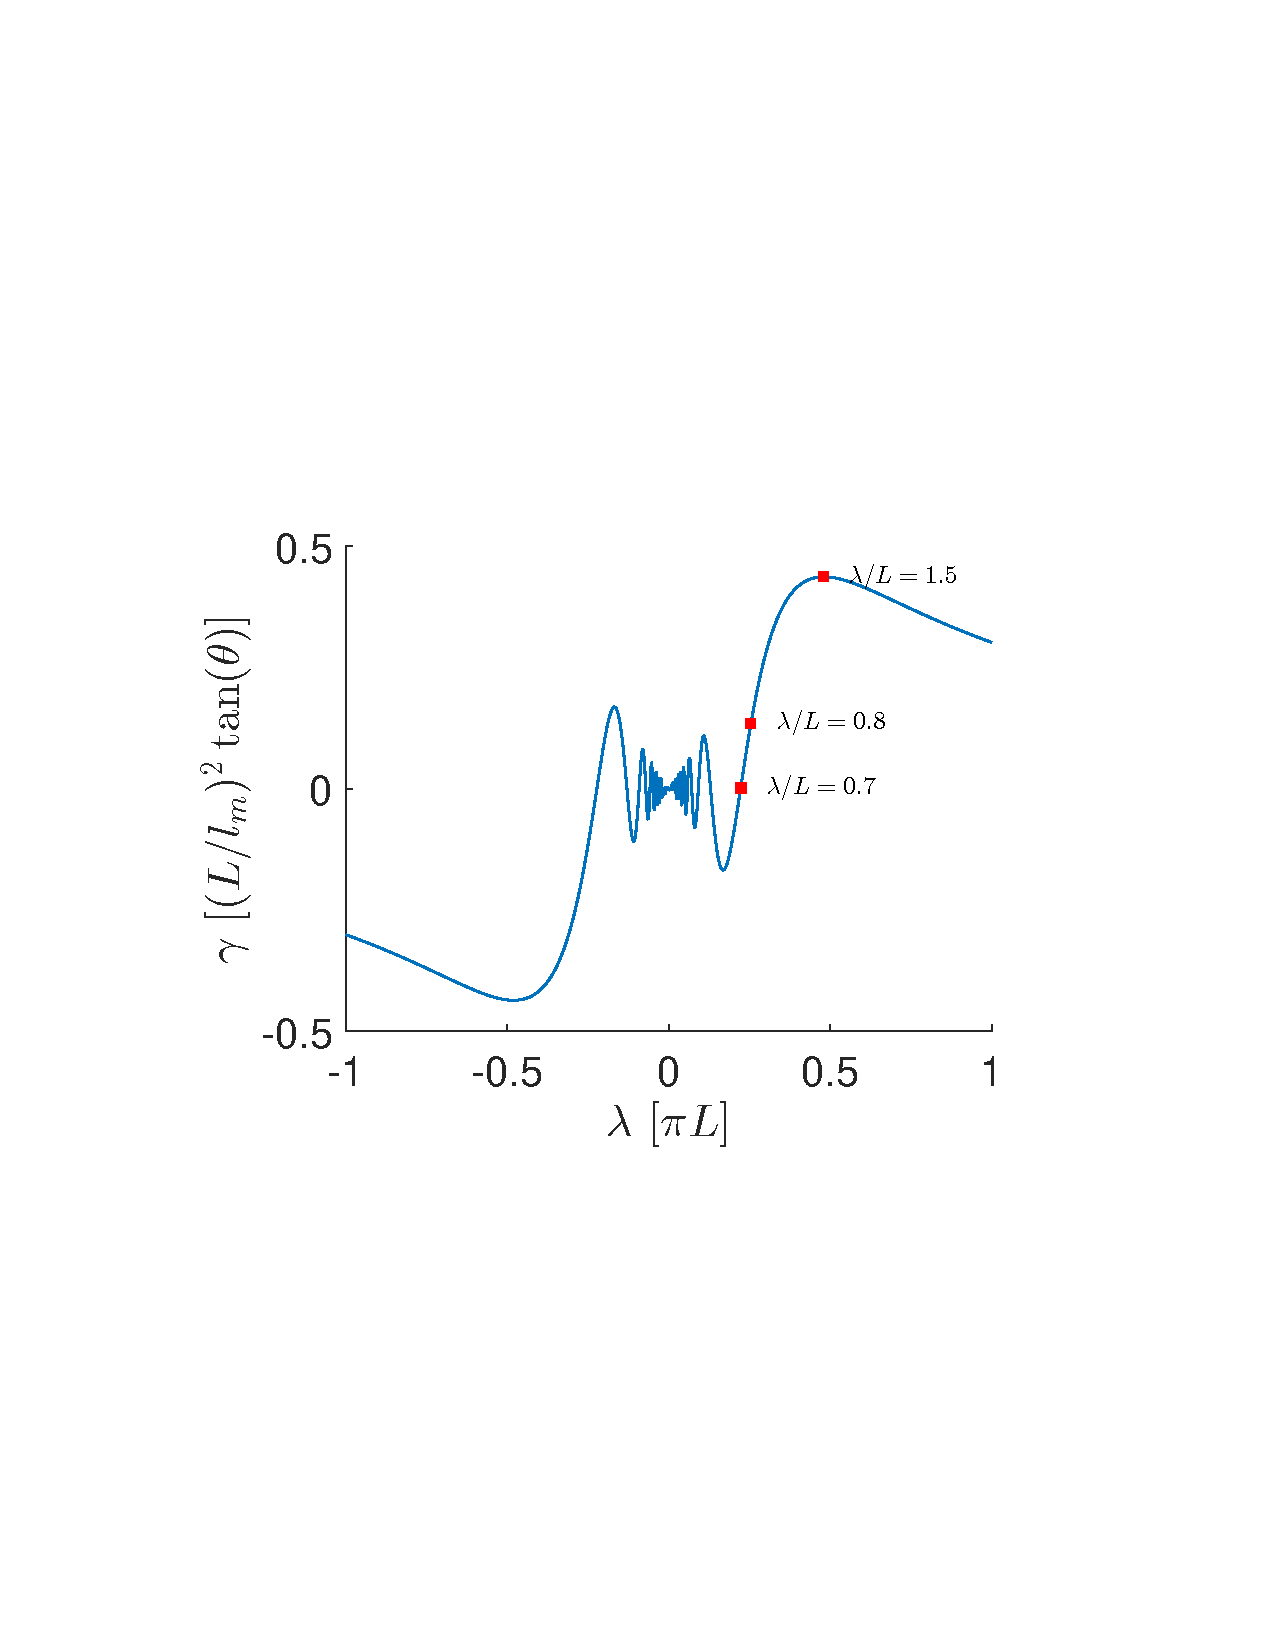
\includegraphics[width=5cm,clip=true,trim=3cm 8cm 4cm 9cm ]{fig/2Gamma3_l_0-3_phi_0}\label{fig:Dist3a}}
\hfill
\subfigure[]{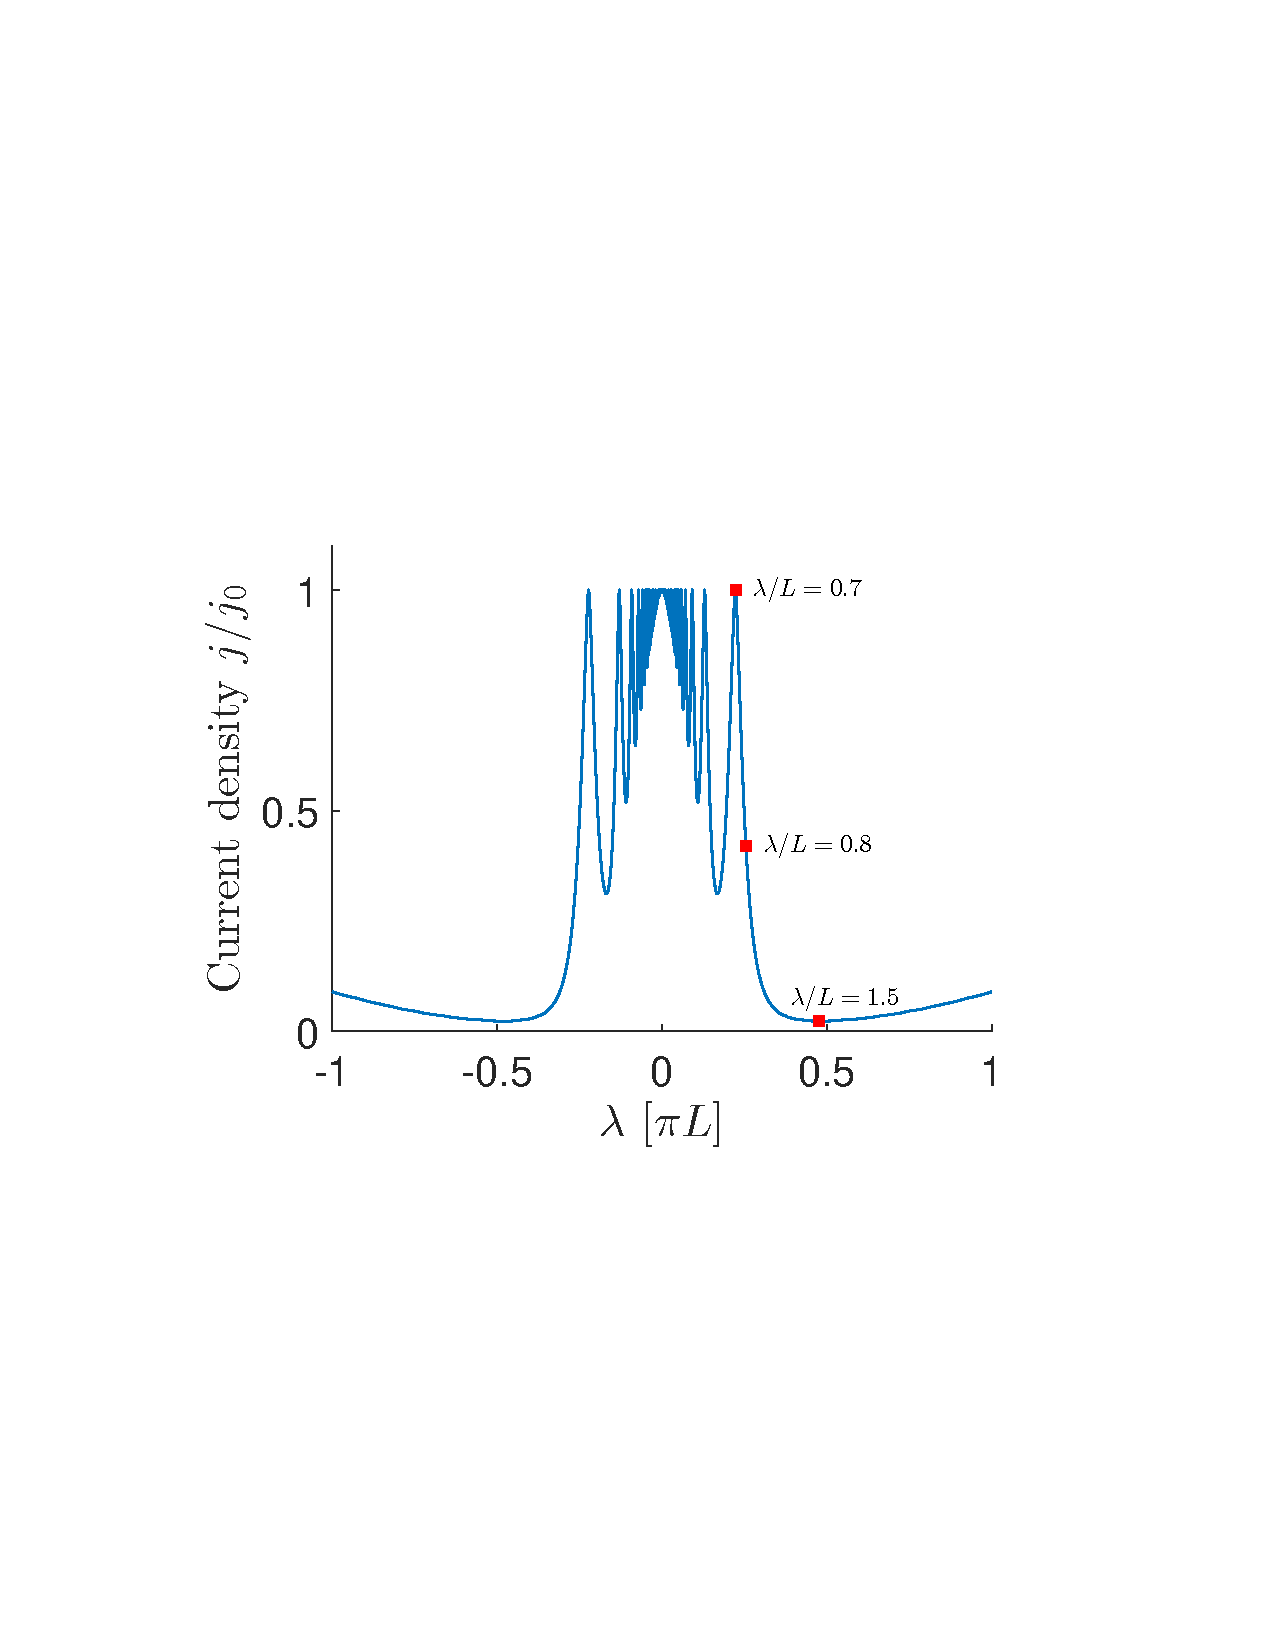
\includegraphics[width=5cm,clip=true,trim=3cm 8cm 4cm 9cm ]{fig/2Dist3_l_0-3_phi_0}\label{fig:Dist3b}}
\hfill
\subfigure[]{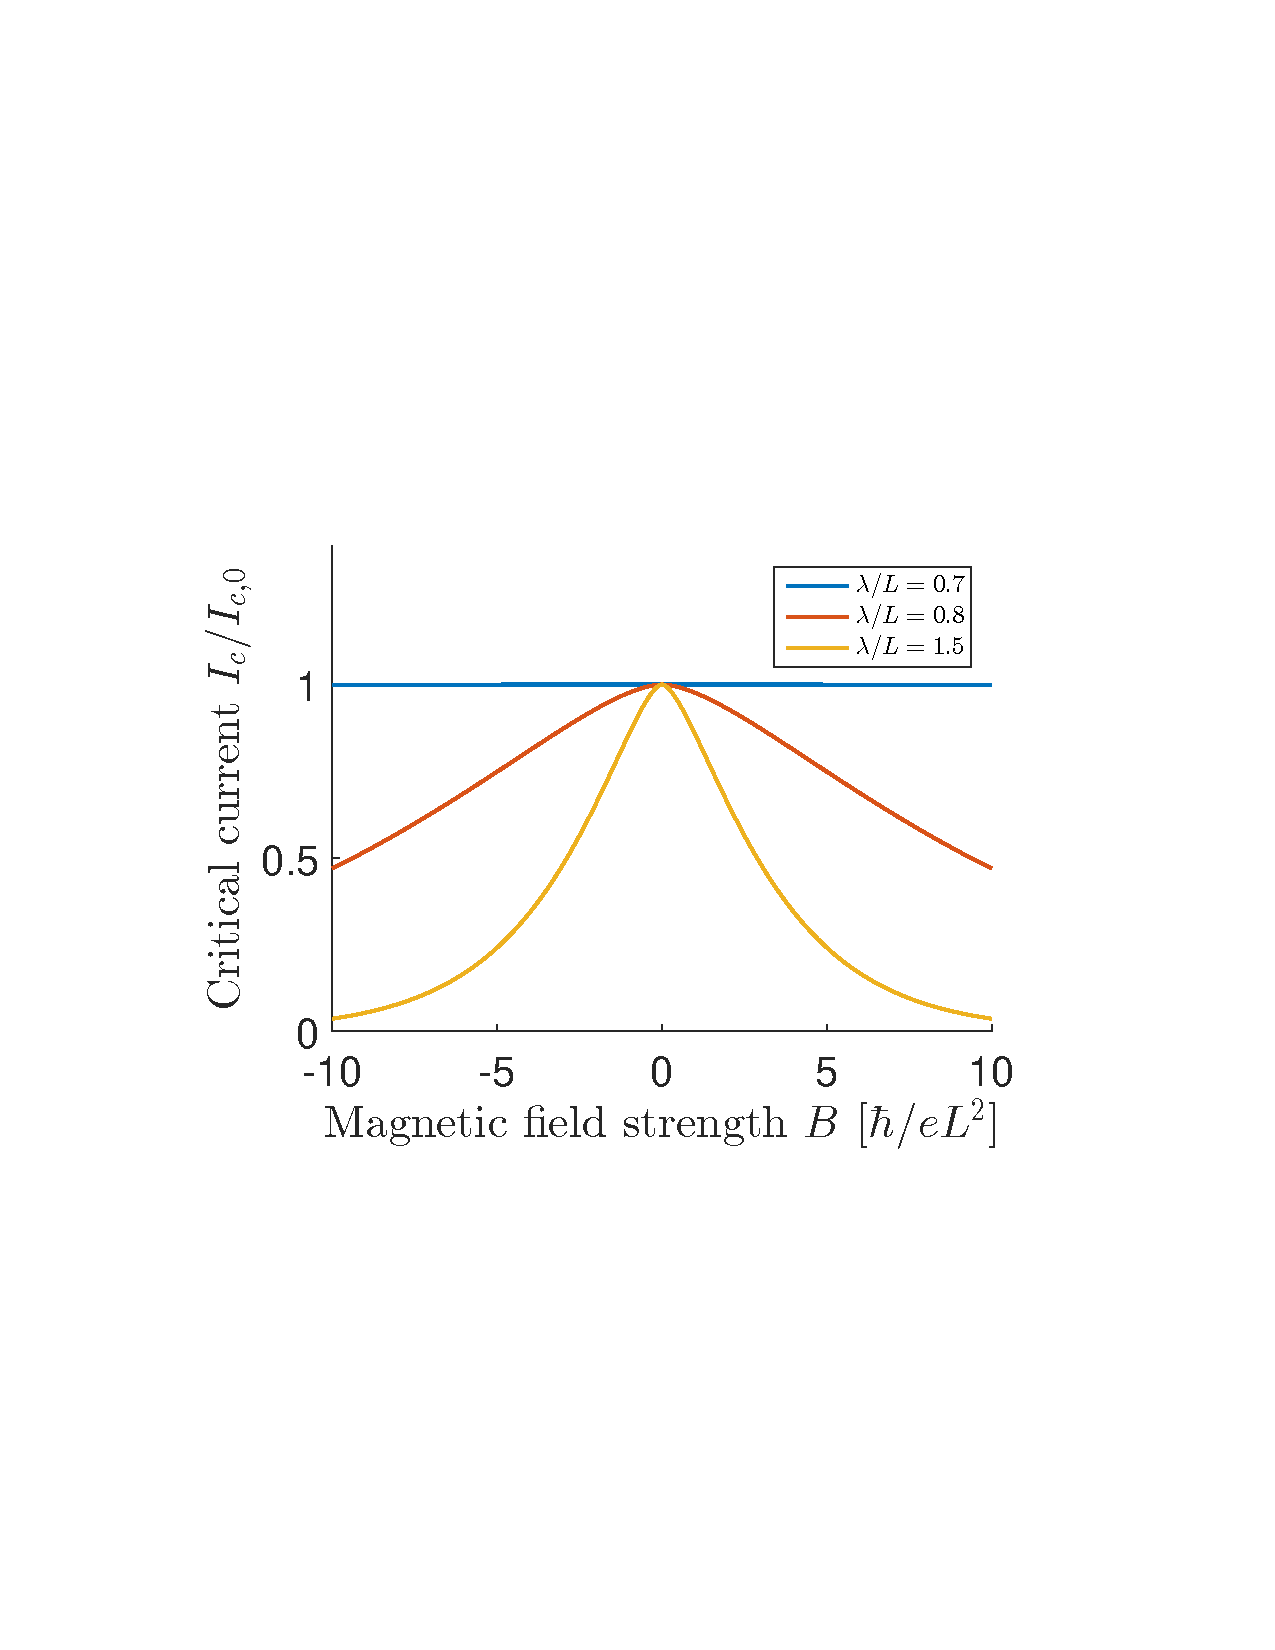
\includegraphics[width=5cm,clip=true,trim=3cm 8cm 4cm 9cm ]{fig/critical_phi_0}\label{fig:Dist3c}}
\caption{blabla}
\label{fig:motionEarth}
\end{figure}

\subsubsection{Symmetric field}
With $\varphi = \pi/2$ in equation \eqref{gamma2} we get
\begin{equation}
\gamma= \frac{2\lambda}{\pi l_m^2}\left[y_0 - x_0\tan\theta_k\right]\sin\left(\frac{\pi L}{\lambda}\right) = \gamma_{\mathrm{const}}\frac{\sin\left(\pi L/\lambda\right)}{\pi L/\lambda}
\end{equation}
where $\gamma_{\mathrm{const}}$ is the Aharonov-Bohm phase shift in a constant magnetic field as given in equation \eqref{gamma1}. We use this expression in equation \eqref{dIwithB} and \eqref{CurrentDensity}, and find the current density numerically. The result is shown in figure \ref{fig:Dist2} for three different wavelengths. 
\begin{figure}[hhh]
\centering
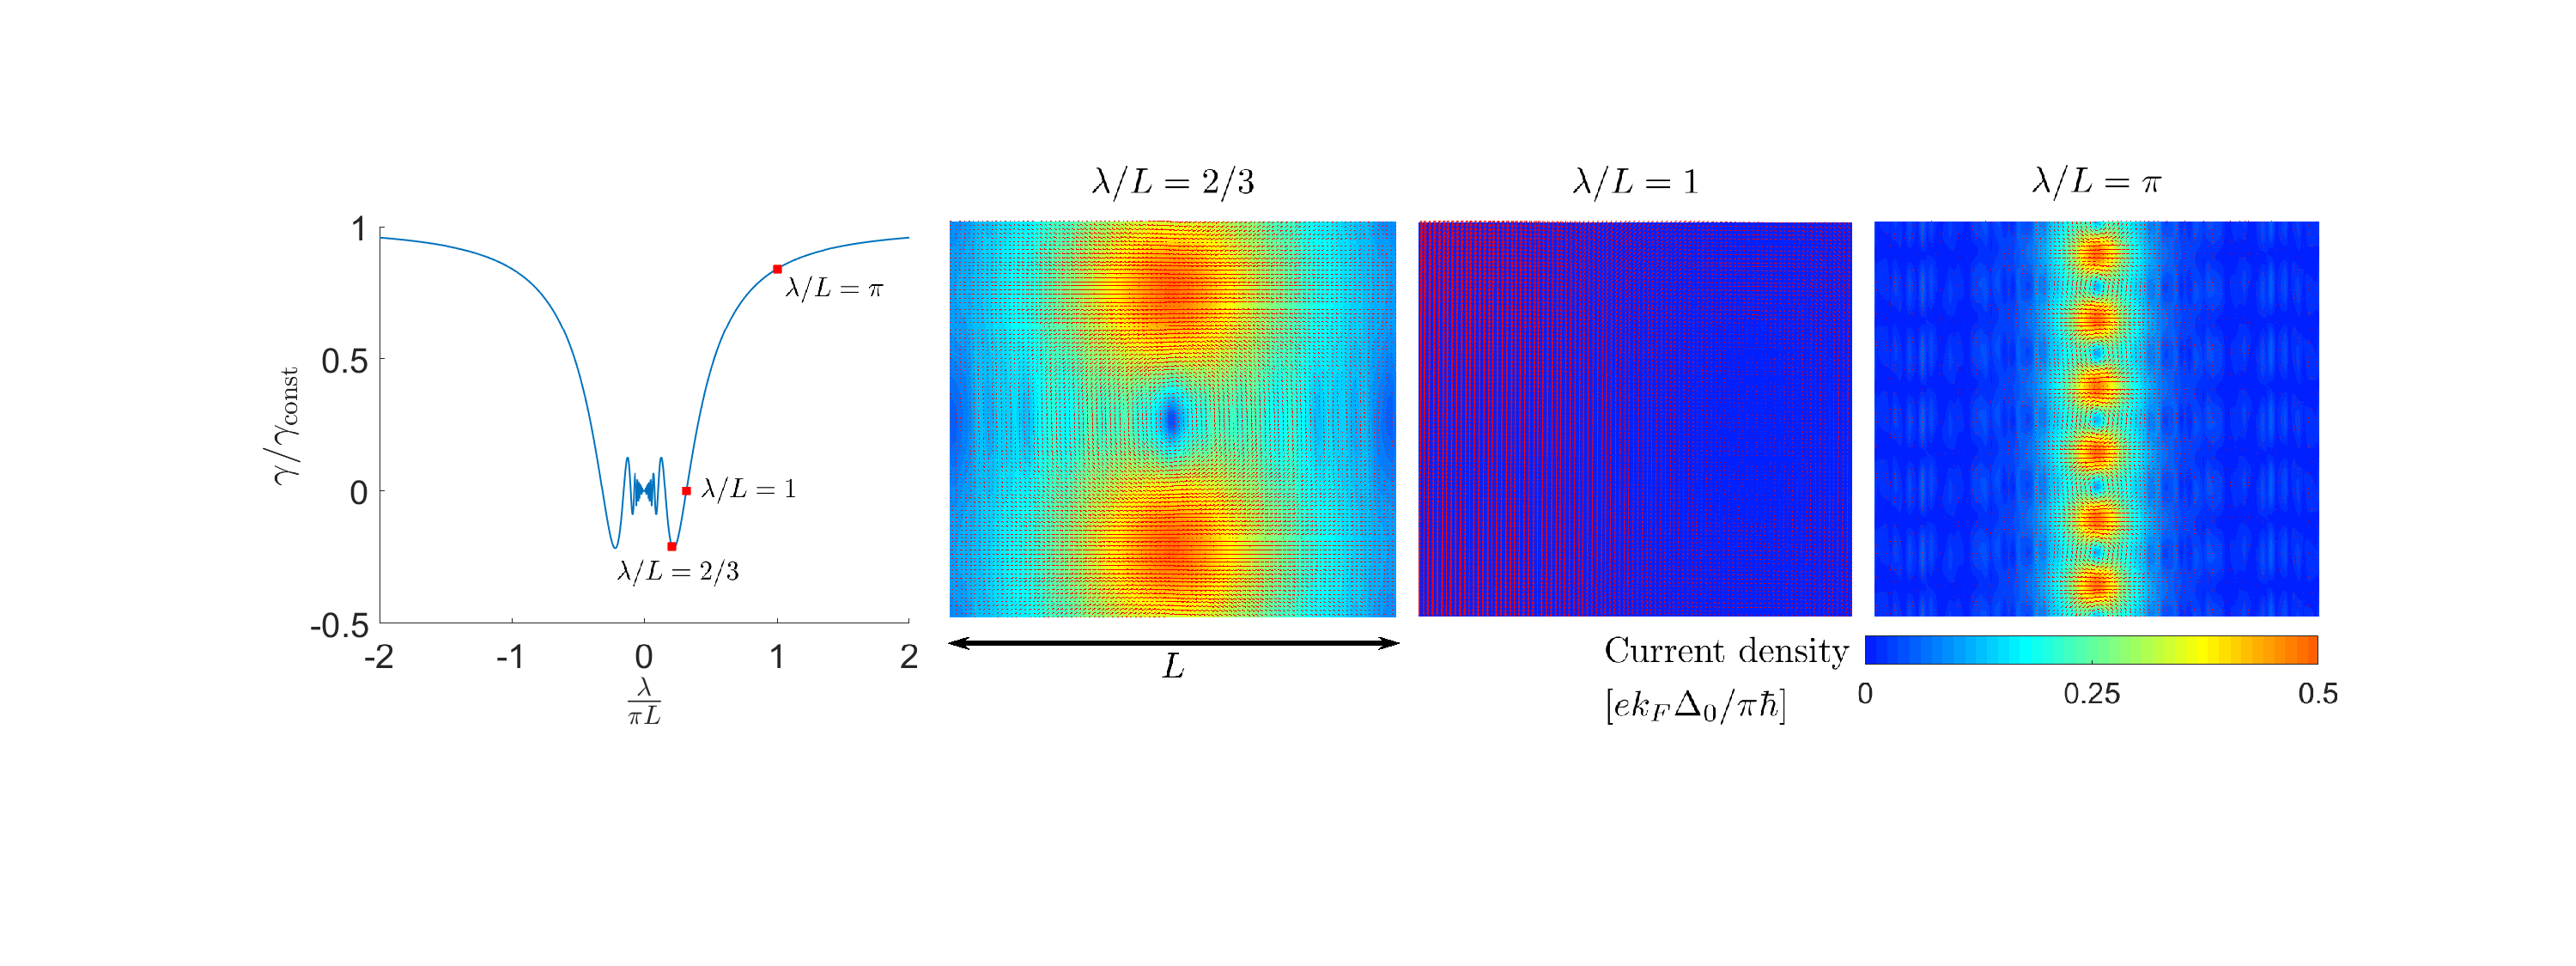
\includegraphics[width=17cm,clip=true,trim=5cm 4.5cm 4.4cm 3cm]{fig/dist3_pi-2}
%\subfigure[]{\includegraphics[width=3.9cm]{Dustin}\label{fig:Dustin}}
%\hfill
%\subfigure[]{\includegraphics[width=3.45cm]{Martin}\label{fig:Martin}}
\caption{blabla}
\label{fig:Dist2}
\end{figure}
\\
\\
The total current is found in the same manner as in section  \ref{sec:ConstField}, giving
\begin{equation}
I_x = I_{c,0}\sin(\Delta \varphi)\frac{\sin\left(\frac{LW}{l_m^2}\frac{\sin(\pi L/\lambda)}{\pi L/\lambda}\right)}{\frac{LW}{l_m^2}\frac{\sin(\pi L/\lambda)}{\pi L/\lambda}} = I_{c,0}\sin\Delta\varphi\frac{\sin(\frac{e}{\hbar}\Phi)}{\frac{e}{\hbar}\Phi}
\end{equation}
where $\Phi$ is the magnetic flux:
\begin{equation}
    \Phi = \int \fet{B}\cdot d\fet{A} = \int \int B\cos\left(\frac{2\pi}{\lambda}x\right)dxdy = \Phi_{\mathrm{const}}\frac{\sin(\pi L/\lambda)}{\pi L/\lambda},
\end{equation}
with $\Phi_{\mathrm{const}} = BWL$ as the magnetic flux in a constant field. In terms of magnetic flux the total current is the same as obtained for constant field, with critical current
\begin{equation}
    I_c = I_{c,0}\frac{\sin(\frac{e}{\hbar}\Phi)}{\frac{e}{\hbar}\Phi}.
\end{equation}
However, the flux, and hence the critical current, is dependent on the wavelength, $\lambda$. In figure \ref{fig:critical_phi_pi-2} the critical current for three different wavelengths is shown for varying field strength, $B$. 
\begin{figure}[hhh]
\centering
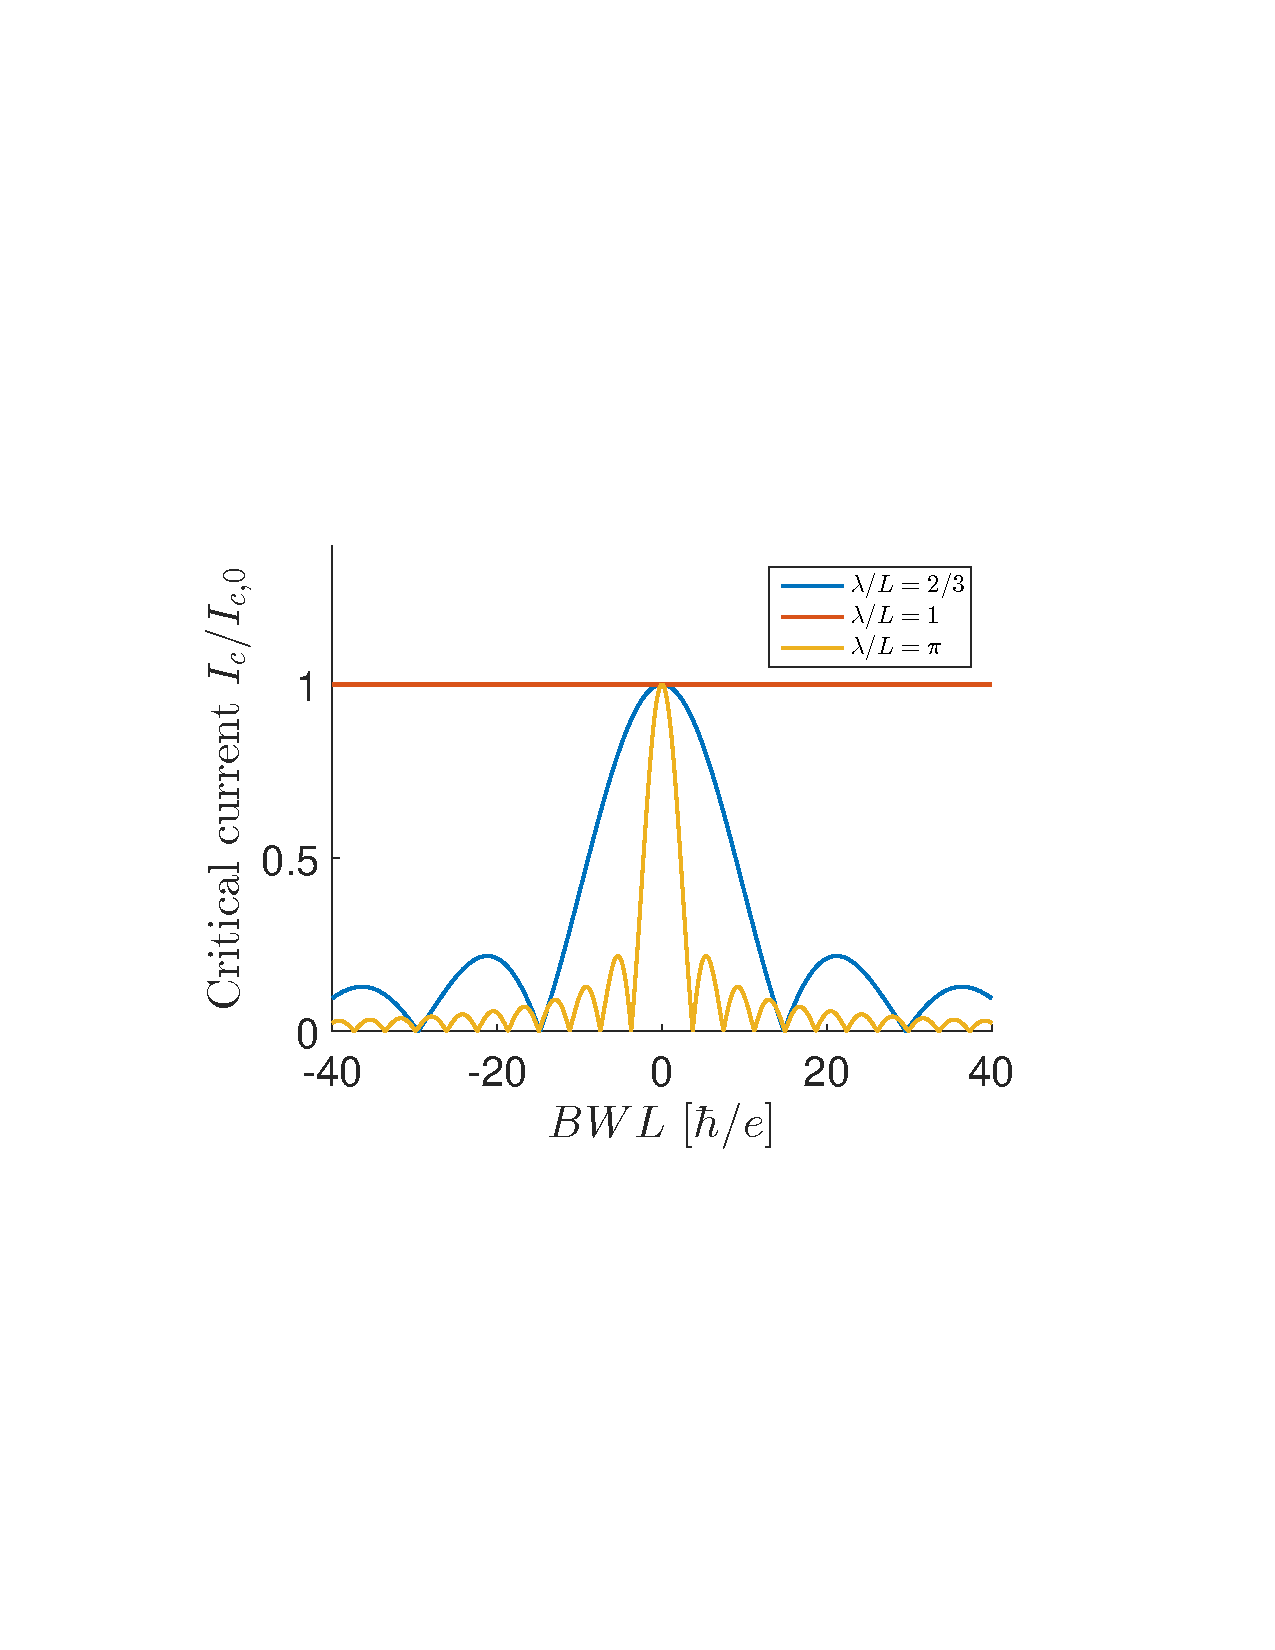
\includegraphics[width=8cm,clip=true,trim=3cm 8cm 4cm 9cm]{fig/critical_phi_pi-2}
%\subfigure[]{\includegraphics[width=3.9cm]{Dustin}\label{fig:Dustin}}
%\hfill
%\subfigure[]{\includegraphics[width=3.45cm]{Martin}\label{fig:Martin}}
\caption{blabla}
\label{fig:critical_phi_pi-2}
\end{figure}

\subsection{Sinusoidal field varying along the interfaces}
Finally we will consider a sinusoidal magnetic field varying along the interfaces:
\begin{equation}
    \fet{B} = B\sin\left(\frac{2\pi}{\lambda}y + \varphi\right)\left[\Theta(x+L/2) - \Theta(x-L/2) \right]\hat{z}
\label{Binterface}
\end{equation}
with the gauge
\begin{equation}
    \fet{A} = B\frac{\lambda}{2\pi}\cos\left(\frac{2\pi}{\lambda}y+\varphi\right)\left[\Theta(x+L/2) - \Theta(x-L/2) \right]\hat{x}.
\end{equation}
This time we find $\gamma$ to be
\begin{equation}
\begin{split}
    \gamma &= 
    %\frac{2}{l_m^2}\frac{\lambda}{2\pi}\int \cos\left(\frac{2\pi}{\lambda}y(x) + \varphi \right) dx =
    \frac{\lambda}{\pi l_m^2 \tan\theta_k}\int_{y_L}^{y_R} \cos\left(\frac{2\pi}{\lambda}y + \varphi \right) dy
    \\
    &= -\frac{\lambda^2}{l_m^2\pi^2\tan\theta_k}\sin\left(\frac{\pi L}{\lambda}\tan\theta_k\right)\cos\left(\frac{2\pi}{\lambda}\left[y_0-x_0\tan\theta_k\right] + \varphi\right).
\end{split}
\end{equation}

\subsubsection{Anti-symmetric field}
With $\varphi = 0$ the expression reads
\begin{equation}
    \gamma = -\frac{L^2}{l_m^2}\frac{\lambda}{\pi L }\frac{\sin\left(\frac{\pi L}{\lambda}\tan\theta_k\right)}{\frac{\pi L}{\lambda}\tan\theta_k}\cos\left(\frac{2\pi}{\lambda}\left[y_0-x_0\tan\theta_k\right]\right).
\end{equation}
The current density is found numerically from equation \eqref{dIwithB} and \eqref{CurrentDensity}. The result is shown in figure \ref{fig:dist2_0} for five different wavelengths. 
\begin{figure}[hhh]
\centering
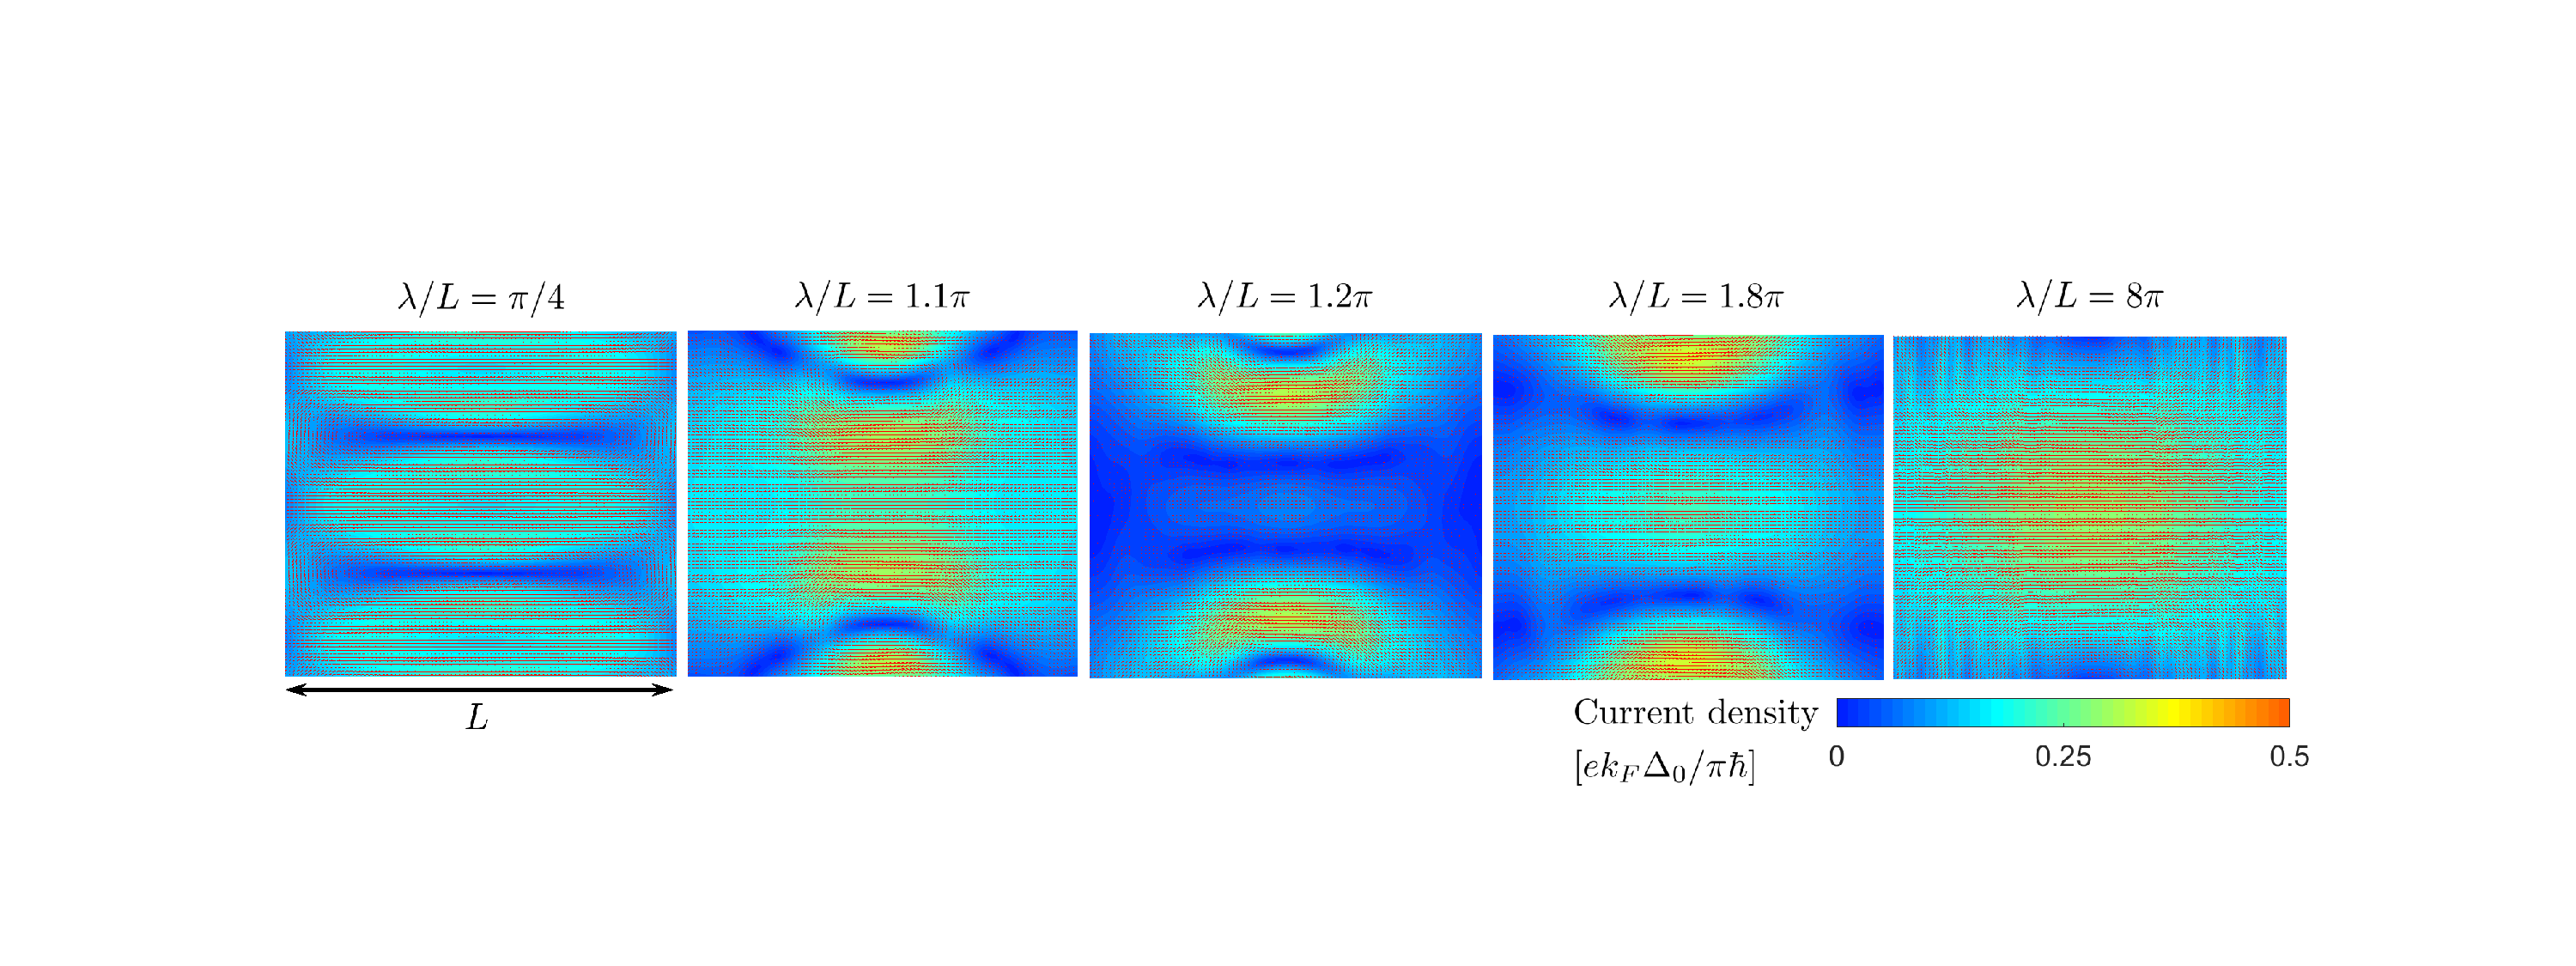
\includegraphics[width=17cm,clip=true,trim = 5.5cm 3.5cm 5cm 5cm]{fig/dist2_0}
%\subfigure[]{\includegraphics[width=3.9cm]{Dustin}\label{fig:Dustin}}
%\hfill
%\subfigure[]{\includegraphics[width=3.45cm]{Martin}\label{fig:Martin}}
\caption{blabla}
\label{fig:dist2_0}
\end{figure}
\\
From equation \eqref{dIwithB} and \eqref{TotalCurrent}, and using that $\gamma(x_0,y_0,\theta_k) = \gamma(x_0,-y_0,-\theta_k)$ we find the total current in the high temperature regime to be
\begin{equation}
I = I_{c,0}\left(J_1\sin\Delta\varphi  - J_2\cos\Delta\varphi\right)
\end{equation}
where $J_1$ and $J_2$ are defined as
\begin{equation}
\begin{split}
    J_1 &\equiv \frac{1}{W}\int_{-W/2}^{W/2}dy_0\int_0^{\pi/2}d\theta_k\cos\theta_k\cos\gamma \\
    J_2 &\equiv \frac{1}{W}\int_{-W/2}^{W/2}dy_0\int_0^{\pi/2}d\theta_k\cos\theta_k\sin\gamma.
\end{split}
\end{equation}
The second integral, $J_2$, is zero (BUT WHY?), and hence the total and critical current is on the same form as for the other cases. The critical current is given as
\begin{equation}
    I_c = \frac{I_{c,0}}{W}\int_{-W/2}^{W/2}dy_0\int_0^{\pi/2}d\theta_k\cos\theta_k\cos\gamma. \\
\end{equation}
\begin{comment}
The critical current is found at $\Delta\varphi = -\arctan(J_1 / J_2)$:
\begin{equation}
    I_c = I_{c,0}\sqrt{J_1^2+J_2^2}.
\end{equation}
\end{comment}
As the expression for $\gamma$ is quite complicated we can not calculate the integral analytically. However, the critical current is found numerically and the result is shown in figure \ref{fig:critical_Dist2_phi_0}.
\begin{figure}[hhh]
\centering
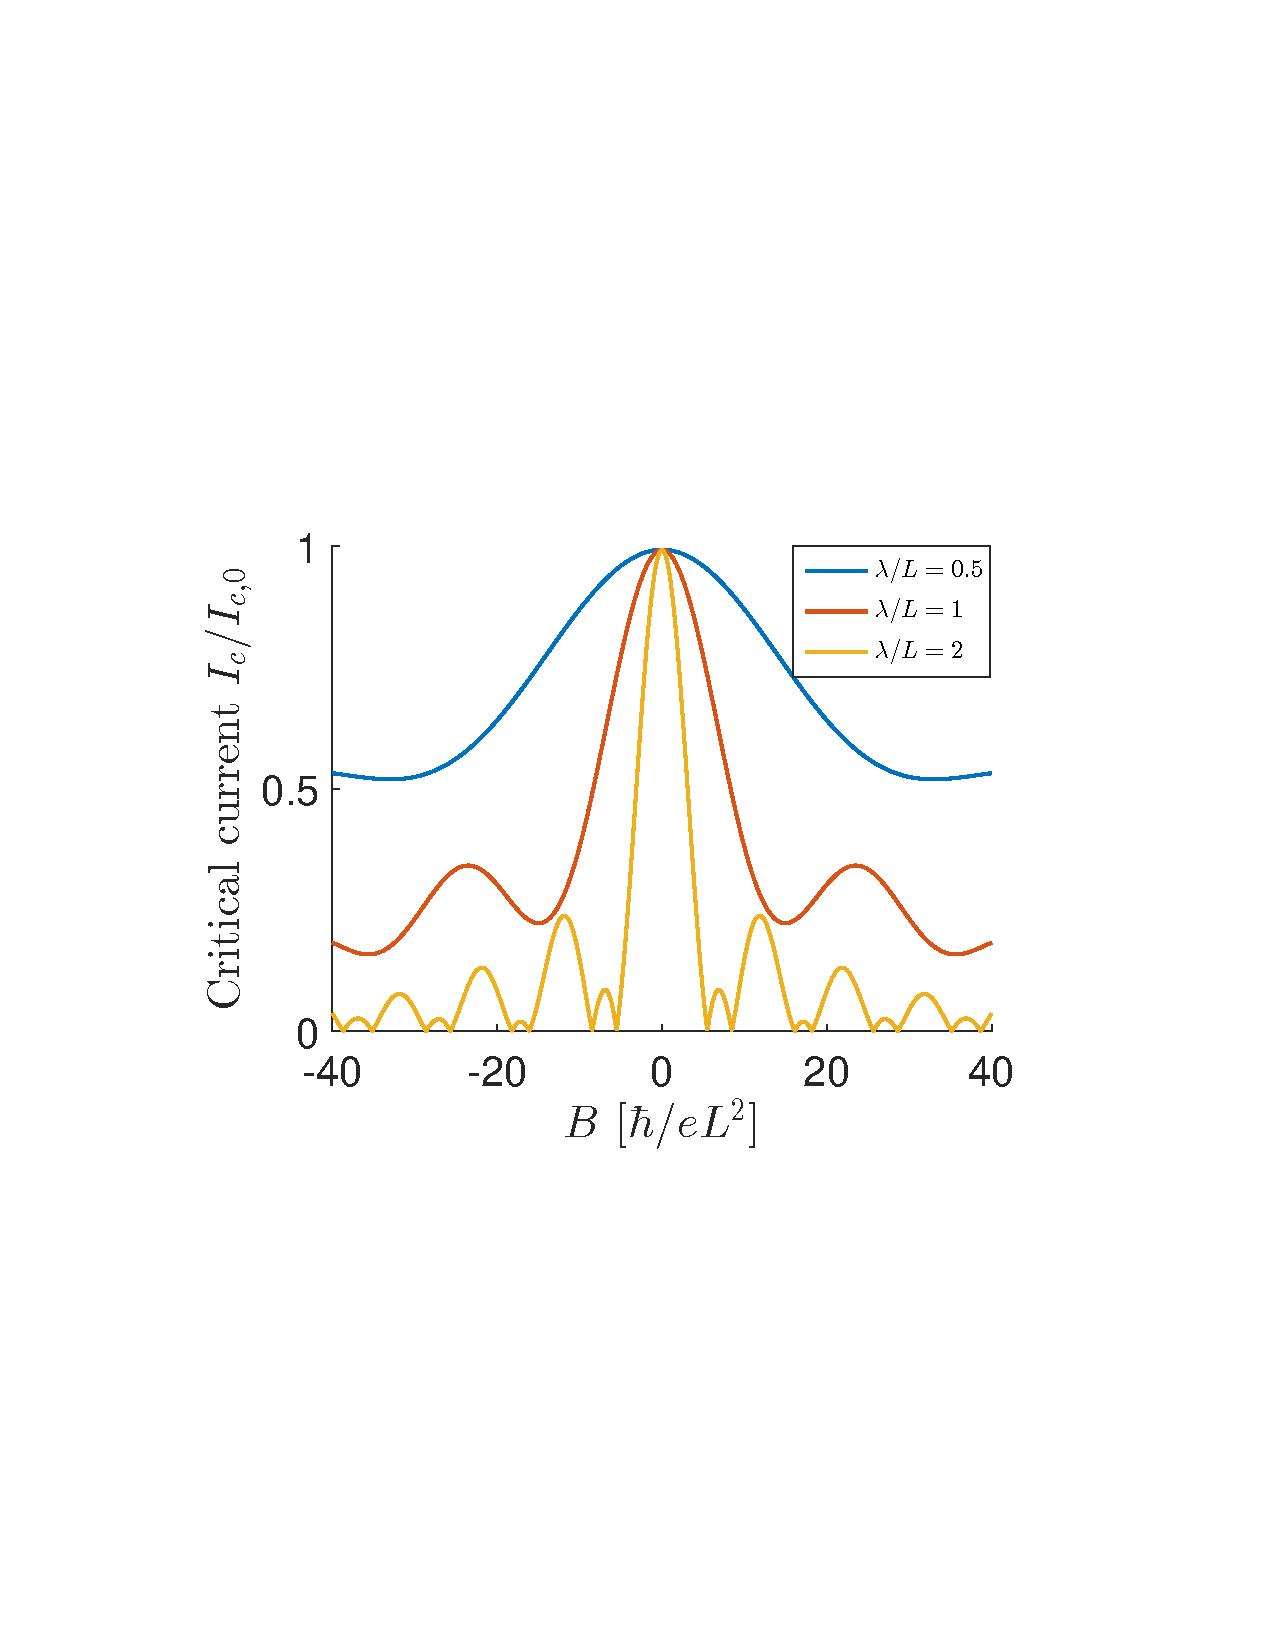
\includegraphics[width=8cm,clip=true,trim=3cm 8cm 4cm 9cm]{fig/critical_Dist2_phi_0}
%\subfigure[]{\includegraphics[width=3.9cm]{Dustin}\label{fig:Dustin}}
%\hfill
%\subfigure[]{\includegraphics[width=3.45cm]{Martin}\label{fig:Martin}}
\caption{blabla}
\label{fig:critical_Dist2_phi_0}
\end{figure}


\subsubsection{Symmetric field}
We $\varphi =\pi/2$ in equation \eqref{Binterface} to obtain a symmetric field and equation \eqref{gamma3} gives
\begin{equation}
\begin{split}
    \gamma &= -\frac{\lambda^2}{l_m^2\pi^2\tan\theta_k}\sin\left(\frac{\pi L}{\lambda}\tan\theta_k\right)\sin\left(\frac{2\pi}{\lambda}\left[y_0-x_0\tan\theta_k\right]\right). 
    \\
    &= -\gamma_{\mathrm{const}}\frac{\sin\left(\frac{\pi L}{\lambda}\tan\theta_k\right)}{\frac{\pi L}{\lambda}\tan\theta_k}\frac{\sin\left(\frac{2\pi}{\lambda}\left[y_0-x_0\tan\theta_k\right]\right)}{\frac{2\pi}{\lambda}\left[y_0-x_0\tan\theta_k\right]}.
\end{split}
\end{equation}
The current density is found numerically and the result is shown in figure \ref{fig:dist2_pi-2}.
\begin{figure}[hhh]
\centering
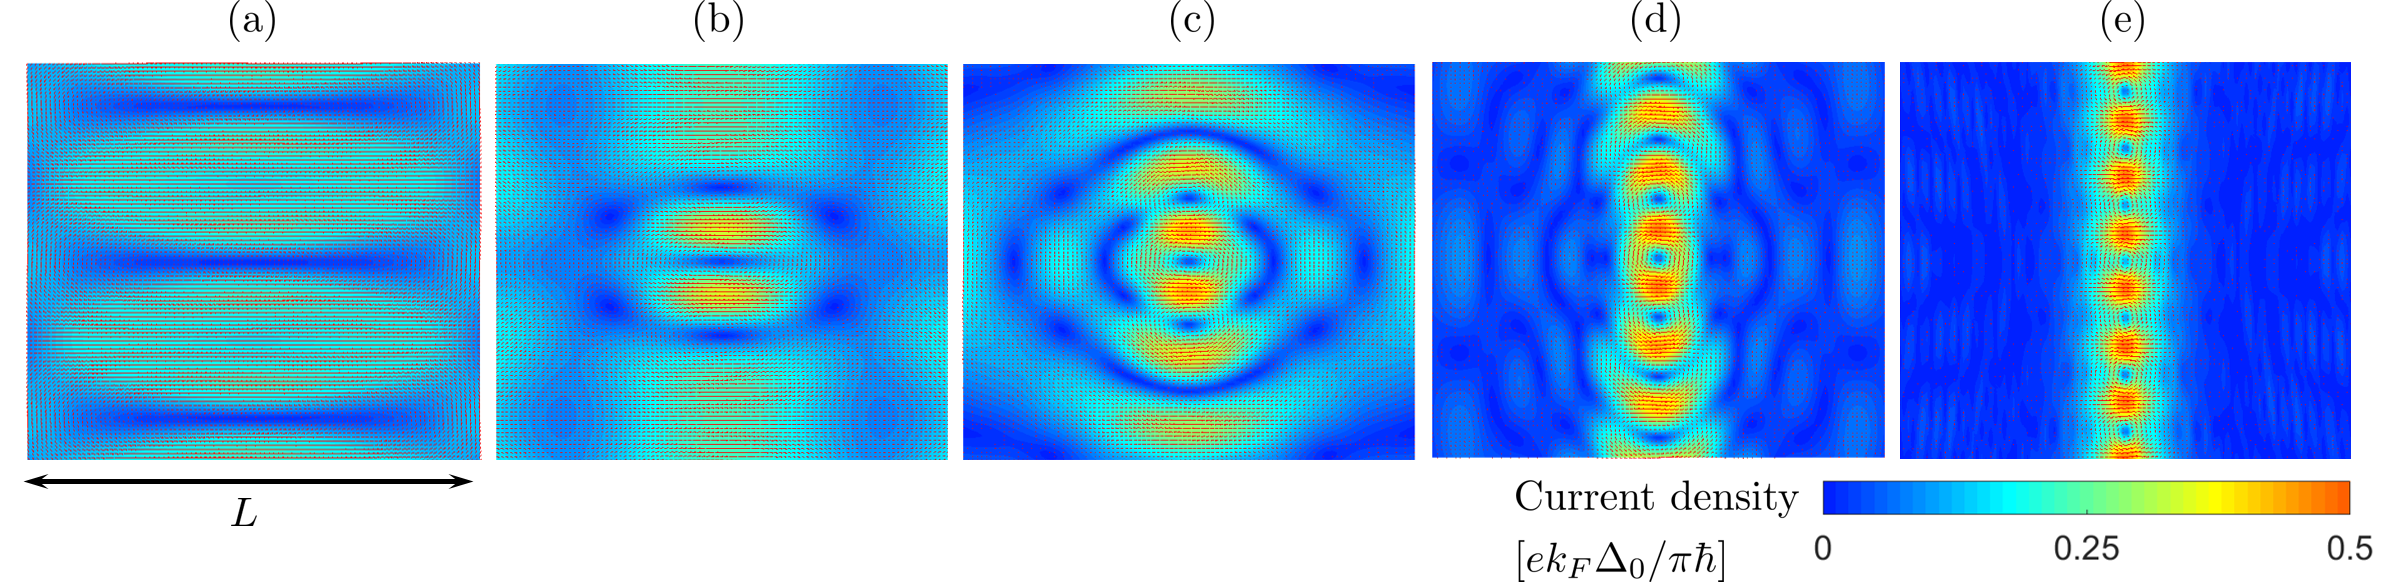
\includegraphics[width=17cm]{fig/dist2pi-2}
%\subfigure[]{\includegraphics[width=3.9cm]{Dustin}\label{fig:Dustin}}
%\hfill
%\subfigure[]{\includegraphics[width=3.45cm]{Martin}\label{fig:Martin}}
\caption{blabla}
\label{fig:dist2_pi-2}
\end{figure}
From equation \eqref{dIwithB} and \eqref{CurrentDensity}, and using that $\gamma(x_0,y_0,\theta_k) = -\gamma(x_0,-y_0,-\theta_k)$ one find the total current to be given as
\begin{equation}
    I = \frac{I_{c,0}}{W}\sin\Delta\varphi\int_{-W/2}^{W/2}dy_0\int_0^{\pi/2}d\theta\cos\theta_k\cos\gamma
\end{equation}
and hence critical current
\begin{equation}
    I_c = \frac{I_{c,0}}{W}\int_{-W/2}^{W/2}dy_0\int_0^{\pi/2}d\theta\cos\theta_k\cos\gamma.
\end{equation}
Again we can only solve the integral numerically and the result of the critical current is shown in figure \ref{fig:critical_dist2_pi-2}.

\begin{figure}[hhh]
\centering
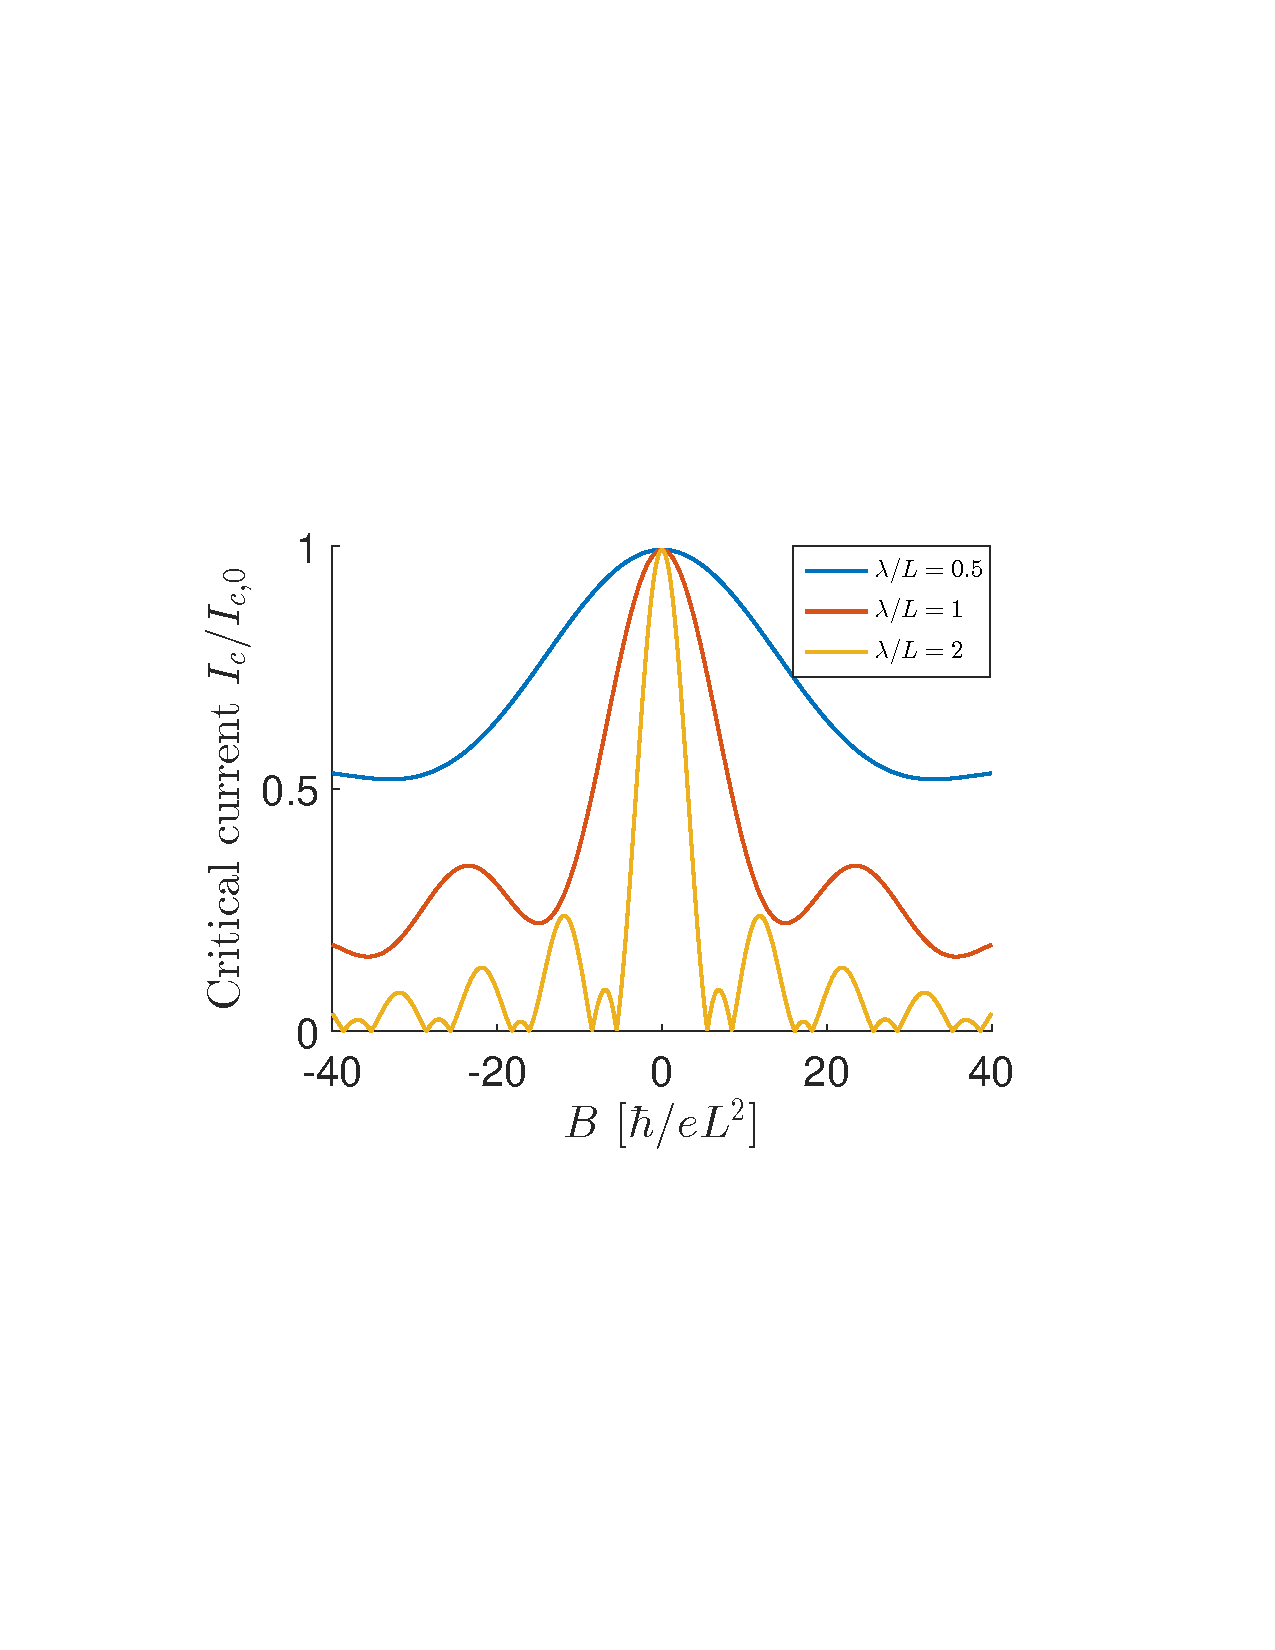
\includegraphics[width=8cm,clip=true,trim=3cm 8cm 4cm 9cm]{fig/critical_Dist2_phi_pi-2}
%\subfigure[]{\includegraphics[width=3.9cm]{Dustin}\label{fig:Dustin}}
%\hfill
%\subfigure[]{\includegraphics[width=3.45cm]{Martin}\label{fig:Martin}}
\caption{blabla}
\label{fig:critical_dist2_pi-2}
\end{figure}